%\VignetteIndexEntry{MAST-intro}
%\VignetteEngine{knitr::knitr}
\documentclass{article}\usepackage[]{graphicx}\usepackage[usenames,dvipsnames]{color}
%% maxwidth is the original width if it is less than linewidth
%% otherwise use linewidth (to make sure the graphics do not exceed the margin)
\makeatletter
\def\maxwidth{ %
  \ifdim\Gin@nat@width>\linewidth
    \linewidth
  \else
    \Gin@nat@width
  \fi
}
\makeatother

\definecolor{fgcolor}{rgb}{0.251, 0.251, 0.251}
\newcommand{\hlnum}[1]{\textcolor[rgb]{0.816,0.125,0.439}{#1}}%
\newcommand{\hlstr}[1]{\textcolor[rgb]{0.251,0.627,0.251}{#1}}%
\newcommand{\hlcom}[1]{\textcolor[rgb]{0.502,0.502,0.502}{\textit{#1}}}%
\newcommand{\hlopt}[1]{\textcolor[rgb]{0,0,0}{#1}}%
\newcommand{\hlstd}[1]{\textcolor[rgb]{0.251,0.251,0.251}{#1}}%
\newcommand{\hlkwa}[1]{\textcolor[rgb]{0.125,0.125,0.941}{#1}}%
\newcommand{\hlkwb}[1]{\textcolor[rgb]{0,0,0}{#1}}%
\newcommand{\hlkwc}[1]{\textcolor[rgb]{0.251,0.251,0.251}{#1}}%
\newcommand{\hlkwd}[1]{\textcolor[rgb]{0.878,0.439,0.125}{#1}}%
\let\hlipl\hlkwb

\newenvironment{knitrout}{}{} % an empty environment to be redefined in TeX
\usepackage{alltt}
\RequirePackage[]{/Library/Frameworks/R.framework/Versions/3.4/Resources/library/BiocStyle/resources/tex/Bioconductor2}
\AtBeginDocument{\bibliographystyle{/Library/Frameworks/R.framework/Versions/3.4/Resources/library/BiocStyle/resources/tex/unsrturl}}

\usepackage{url}
\usepackage{color}
\usepackage[cm]{fullpage}
\usepackage[usenames,dvipsnames]{xcolor}
\usepackage{comment}
\usepackage{doi}
\usepackage{amsmath}
%\usepackage[authoryear]{natbib}

%\makeatletter
%%%%%%%%%%%%%%%%%%%%%%%%%%%%%% User specified LaTeX commands.
% \VignetteIndexEntry{An Introduction to SingleCellAssay}

%\makeatother
\newcommand{\future}[1]{TODO: {\color{gray} #1}}
\newcommand{\sca}{\texttt{SingleCellAssay}}
\newcommand{\mast}{\texttt{MAST}}
\input{symbols.tex}
\IfFileExists{upquote.sty}{\usepackage{upquote}}{}
\begin{document}
\title{An Introduction to MAST}


\author{Andrew McDavid and Greg Finak}

\maketitle
\section{Philosophy}
 \mast is an R/Bioconductor package for managing and analyzing qPCR and sequencing-based single--cell gene expression
 data, as well as data from other types of single--cell assays. 
Our goal is to support assays that have multiple \emph{features} (genes,
markers, etc) per \emph{well} (cell, etc) in a flexible manner.
Assays are assumed to be  mostly \emph{complete} in the sense that most \emph{wells}
contain measurements for all features.

\subsection{Internals}
A \texttt{SingleCellAssay} object can be manipulated as a matrix, with rows giving features and columns giving cells.
It derives from \href{http://bioconductor.org/packages/release/bioc/html/SummarizedExperiment.html}{\texttt{SummarizedExperiment}}.

\subsection{Statistical Testing}
Apart from reading and storing single--cell assay data, the package also
provides functionality for significance testing of differential expression using a Hurdle model, gene set enrichment, facilities for visualizing patterns in residuals indicative of differential expression, and power calculations (soon).

There is also some facilities for inferring background thresholds, and filtering of individual outlier wells/libraries. 
These methods are described our papers. 
% Add citations

\section{Examples}

With the cursory background out of the way, we'll proceed with some examples
to help understand how the package is used.

\subsection{Reading Data}
Data can be imported in a Fluidigm instrument-specific format (the details of
which are undocumented, and likely subject-to-change) or some derived,
annotated format,  or in ``long'' (melted) format, in which each row is a
measurement, so if there are $N$ wells and $M$ cells, then the
\texttt{data.frame} should contain $N \times M$ rows.

For example, the following data set was provided in as a comma-separated value file.
It has the cycle threshold ($\ct$) recorded. 
Non-detected genes are recorded as NAs.
For the Fluidigm/qPCR single cell expression functions to work as expected, we
must use the \emph{expression threshold}, defined as $et = c_{\mbox{max}} - \ct$, which is proportional to the log-expression.

Below, we load the package and the data, then compute the expression threshold from the $\ct$, and construct a \texttt{FluidigmAssay}.
\begin{knitrout}
\definecolor{shadecolor}{rgb}{0.941, 0.941, 0.941}\color{fgcolor}\begin{kframe}
\begin{alltt}
\hlkwd{library}\hlstd{(MAST)}
\end{alltt}


{\ttfamily\noindent\itshape\color{messagecolor}{\#\# Loading required package: SummarizedExperiment}}

{\ttfamily\noindent\itshape\color{messagecolor}{\#\# Loading required package: GenomicRanges}}

{\ttfamily\noindent\itshape\color{messagecolor}{\#\# Loading required package: stats4}}

{\ttfamily\noindent\itshape\color{messagecolor}{\#\# Loading required package: BiocGenerics}}

{\ttfamily\noindent\itshape\color{messagecolor}{\#\# Loading required package: parallel}}

{\ttfamily\noindent\itshape\color{messagecolor}{\#\# \\\#\# Attaching package: 'BiocGenerics'}}

{\ttfamily\noindent\itshape\color{messagecolor}{\#\# The following objects are masked from 'package:parallel':\\\#\# \\\#\#\ \ \ \  clusterApply, clusterApplyLB, clusterCall, clusterEvalQ,\\\#\#\ \ \ \  clusterExport, clusterMap, parApply, parCapply, parLapply,\\\#\#\ \ \ \  parLapplyLB, parRapply, parSapply, parSapplyLB}}

{\ttfamily\noindent\itshape\color{messagecolor}{\#\# The following objects are masked from 'package:stats':\\\#\# \\\#\#\ \ \ \  IQR, mad, sd, var, xtabs}}

{\ttfamily\noindent\itshape\color{messagecolor}{\#\# The following objects are masked from 'package:base':\\\#\# \\\#\#\ \ \ \  anyDuplicated, append, as.data.frame, cbind, colMeans, colnames,\\\#\#\ \ \ \  colSums, do.call, duplicated, eval, evalq, Filter, Find, get,\\\#\#\ \ \ \  grep, grepl, intersect, is.unsorted, lapply, lengths, Map,\\\#\#\ \ \ \  mapply, match, mget, order, paste, pmax, pmax.int, pmin,\\\#\#\ \ \ \  pmin.int, Position, rank, rbind, Reduce, rowMeans, rownames,\\\#\#\ \ \ \  rowSums, sapply, setdiff, sort, table, tapply, union, unique,\\\#\#\ \ \ \  unsplit, which, which.max, which.min}}

{\ttfamily\noindent\itshape\color{messagecolor}{\#\# Loading required package: S4Vectors}}

{\ttfamily\noindent\itshape\color{messagecolor}{\#\# \\\#\# Attaching package: 'S4Vectors'}}

{\ttfamily\noindent\itshape\color{messagecolor}{\#\# The following object is masked from 'package:base':\\\#\# \\\#\#\ \ \ \  expand.grid}}

{\ttfamily\noindent\itshape\color{messagecolor}{\#\# Loading required package: IRanges}}

{\ttfamily\noindent\itshape\color{messagecolor}{\#\# Loading required package: GenomeInfoDb}}

{\ttfamily\noindent\itshape\color{messagecolor}{\#\# Loading required package: Biobase}}

{\ttfamily\noindent\itshape\color{messagecolor}{\#\# Welcome to Bioconductor\\\#\# \\\#\#\ \ \ \  Vignettes contain introductory material; view with\\\#\#\ \ \ \  'browseVignettes()'. To cite Bioconductor, see\\\#\#\ \ \ \  'citation("{}Biobase"{})', and for packages 'citation("{}pkgname"{})'.}}

{\ttfamily\noindent\itshape\color{messagecolor}{\#\# Loading required package: DelayedArray}}

{\ttfamily\noindent\itshape\color{messagecolor}{\#\# Loading required package: matrixStats}}

{\ttfamily\noindent\itshape\color{messagecolor}{\#\# \\\#\# Attaching package: 'matrixStats'}}

{\ttfamily\noindent\itshape\color{messagecolor}{\#\# The following objects are masked from 'package:Biobase':\\\#\# \\\#\#\ \ \ \  anyMissing, rowMedians}}

{\ttfamily\noindent\itshape\color{messagecolor}{\#\# \\\#\# Attaching package: 'DelayedArray'}}

{\ttfamily\noindent\itshape\color{messagecolor}{\#\# The following objects are masked from 'package:matrixStats':\\\#\# \\\#\#\ \ \ \  colMaxs, colMins, colRanges, rowMaxs, rowMins, rowRanges}}

{\ttfamily\noindent\itshape\color{messagecolor}{\#\# The following object is masked from 'package:base':\\\#\# \\\#\#\ \ \ \  apply}}

{\ttfamily\noindent\itshape\color{messagecolor}{\#\# \\\#\# Attaching package: 'MAST'}}

{\ttfamily\noindent\itshape\color{messagecolor}{\#\# The following object is masked from 'package:stats':\\\#\# \\\#\#\ \ \ \  filter}}\begin{alltt}
\hlkwd{library}\hlstd{(data.table)}
\end{alltt}


{\ttfamily\noindent\itshape\color{messagecolor}{\#\# \\\#\# Attaching package: 'data.table'}}

{\ttfamily\noindent\itshape\color{messagecolor}{\#\# The following object is masked from 'package:SummarizedExperiment':\\\#\# \\\#\#\ \ \ \  shift}}

{\ttfamily\noindent\itshape\color{messagecolor}{\#\# The following object is masked from 'package:GenomicRanges':\\\#\# \\\#\#\ \ \ \  shift}}

{\ttfamily\noindent\itshape\color{messagecolor}{\#\# The following object is masked from 'package:IRanges':\\\#\# \\\#\#\ \ \ \  shift}}

{\ttfamily\noindent\itshape\color{messagecolor}{\#\# The following objects are masked from 'package:S4Vectors':\\\#\# \\\#\#\ \ \ \  first, second}}\begin{alltt}
\hlkwd{data}\hlstd{(vbeta)}
\hlkwd{colnames}\hlstd{(vbeta)}
\end{alltt}
\begin{verbatim}
##  [1] "Sample.ID"         "Subject.ID"        "Experiment.Number"
##  [4] "Chip.Number"       "Stim.Condition"    "Time"             
##  [7] "Population"        "Number.of.Cells"   "Well"             
## [10] "Gene"              "Ct"
\end{verbatim}
\begin{alltt}
\hlstd{vbeta} \hlkwb{<-} \hlkwd{computeEtFromCt}\hlstd{(vbeta)}
\hlstd{vbeta.fa} \hlkwb{<-} \hlkwd{FromFlatDF}\hlstd{(vbeta,} \hlkwc{idvars}\hlstd{=}\hlkwd{c}\hlstd{(}\hlstr{"Subject.ID"}\hlstd{,} \hlstr{"Chip.Number"}\hlstd{,} \hlstr{"Well"}\hlstd{),}
                          \hlkwc{primerid}\hlstd{=}\hlstr{'Gene'}\hlstd{,} \hlkwc{measurement}\hlstd{=}\hlstr{'Et'}\hlstd{,} \hlkwc{ncells}\hlstd{=}\hlstr{'Number.of.Cells'}\hlstd{,}
                          \hlkwc{geneid}\hlstd{=}\hlstr{"Gene"}\hlstd{,}  \hlkwc{cellvars}\hlstd{=}\hlkwd{c}\hlstd{(}\hlstr{'Number.of.Cells'}\hlstd{,} \hlstr{'Population'}\hlstd{),}
                          \hlkwc{phenovars}\hlstd{=}\hlkwd{c}\hlstd{(}\hlstr{'Stim.Condition'}\hlstd{,}\hlstr{'Time'}\hlstd{),} \hlkwc{id}\hlstd{=}\hlstr{'vbeta all'}\hlstd{,} \hlkwc{class}\hlstd{=}\hlstr{'FluidigmAssay'}\hlstd{)}
\hlkwd{print}\hlstd{(vbeta.fa)}
\end{alltt}
\begin{verbatim}
## class: FluidigmAssay 
## dim: 75 456 
## metadata(0):
## assays(1): Et
## rownames(75): B3GAT1 BAX ... TNFRSF9 TNFSF10
## rowData names(2): Gene primerid
## colnames(456): Sub01 1 A01 Sub01 1 A02 ... Sub02 3 H10 Sub02 3 H11
## colData names(9): Number.of.Cells Population ... Time wellKey
\end{verbatim}
\end{kframe}
\end{knitrout}

We see that the variable \texttt{vbeta} is a \texttt{data.frame} from which we
construct the \texttt{FluidigmAssay} object. 
The \texttt{idvars} is the set of column(s) in \texttt{vbeta} that uniquely
identify a well (globally), the \texttt{primerid} is a column(s) that specify the feature measured at this well.
The \texttt{measurement} gives the column name containing the log-expression
measurement, \texttt{ncells} contains the number of cells (or other
normalizing factor) for the well.
\texttt{geneid}, \texttt{cellvars}, \texttt{phenovars} all specify additional
columns to be included in the \texttt{featureData}, \texttt{phenoData}  and
\texttt{cellData} (\future{wellData}). The output is a \texttt{FluidigmAssay}
object with 456 wells and 75 features. 


We can access the feature--level metadata and the cell--level metadata using
the \texttt{mcols} and \texttt{colData} accessors.

\begin{knitrout}
\definecolor{shadecolor}{rgb}{0.941, 0.941, 0.941}\color{fgcolor}\begin{kframe}
\begin{alltt}
\hlkwd{head}\hlstd{(}\hlkwd{mcols}\hlstd{(vbeta.fa),}\hlnum{3}\hlstd{)}
\end{alltt}
\begin{verbatim}
## DataFrame with 3 rows and 2 columns
##          Gene    primerid
##   <character> <character>
## 1      B3GAT1      B3GAT1
## 2         BAX         BAX
## 3        BCL2        BCL2
\end{verbatim}
\begin{alltt}
\hlkwd{head}\hlstd{(}\hlkwd{colData}\hlstd{(vbeta.fa),}\hlnum{3}\hlstd{)}
\end{alltt}
\begin{verbatim}
## DataFrame with 3 rows and 9 columns
##             Number.of.Cells            Population    ncells Subject.ID
##                   <integer>           <character> <integer>   <factor>
## Sub01 1 A01               1 CD154+VbetaResponsive         1      Sub01
## Sub01 1 A02               1 CD154+VbetaResponsive         1      Sub01
## Sub01 1 A03               1 CD154+VbetaResponsive         1      Sub01
##             Chip.Number        Well Stim.Condition     Time     wellKey
##               <integer> <character>    <character> <factor> <character>
## Sub01 1 A01           1         A01      Stim(SEB)       12 Sub01 1 A01
## Sub01 1 A02           1         A02      Stim(SEB)       12 Sub01 1 A02
## Sub01 1 A03           1         A03      Stim(SEB)       12 Sub01 1 A03
\end{verbatim}
\end{kframe}
\end{knitrout}

We see this gives us the set of genes measured in the assay, or the cell-level
metadata (i.e. the number of cells measured in the well, the population this
cell belongs to, the subject it came from, the chip it was run on, the well
id, the stimulation it was subjected to, and the timepoint for the experiment
this cell was part of). The wellKey are concatenated idvars columns, helping to
ensure consistency when splitting and merging \sca objects. 
\subsection{Importing Matrix Data}
Data can also be imported in matrix format using command \texttt{FromMatrix}, and passing a matrix of expression values and \texttt{DataFrame} coercible cell and feature data.

\subsection{Subsetting, splitting, combining, melting}
It's possible to subset \sca objects by wells and features.
Square brackets (``['') will index on
the first index (features) and by features on the second index (cells).
Integer and boolean and indices may be used, as well as character vectors
naming the wellKey or the feature (via the primerid).
There is also a \texttt{subset} method, which will evaluate its argument in the frame of the \texttt{colData}, hence will subset by wells.
\begin{knitrout}
\definecolor{shadecolor}{rgb}{0.941, 0.941, 0.941}\color{fgcolor}\begin{kframe}
\begin{alltt}
\hlstd{sub1} \hlkwb{<-} \hlstd{vbeta.fa[,}\hlnum{1}\hlopt{:}\hlnum{10}\hlstd{]}
\hlkwd{show}\hlstd{(sub1)}
\end{alltt}
\begin{verbatim}
## class: FluidigmAssay 
## dim: 75 10 
## metadata(0):
## assays(1): Et
## rownames(75): B3GAT1 BAX ... TNFRSF9 TNFSF10
## rowData names(2): Gene primerid
## colnames(10): Sub01 1 A01 Sub01 1 A02 ... Sub01 1 A09 Sub01 1 A10
## colData names(9): Number.of.Cells Population ... Time wellKey
\end{verbatim}
\begin{alltt}
\hlstd{sub2} \hlkwb{<-} \hlkwd{subset}\hlstd{(vbeta.fa, Well}\hlopt{==}\hlstr{'A01'}\hlstd{)}
\hlkwd{show}\hlstd{(sub2)}
\end{alltt}
\begin{verbatim}
## class: FluidigmAssay 
## dim: 75 5 
## metadata(0):
## assays(1): Et
## rownames(75): B3GAT1 BAX ... TNFRSF9 TNFSF10
## rowData names(2): Gene primerid
## colnames(5): Sub01 1 A01 Sub01 2 A01 Sub02 1 A01 Sub02 2 A01 Sub02 3
##   A01
## colData names(9): Number.of.Cells Population ... Time wellKey
\end{verbatim}
\begin{alltt}
\hlstd{sub3} \hlkwb{<-} \hlstd{vbeta.fa[}\hlnum{6}\hlopt{:}\hlnum{10}\hlstd{,} \hlnum{1}\hlopt{:}\hlnum{10}\hlstd{]}
\hlkwd{show}\hlstd{(sub3)}
\end{alltt}
\begin{verbatim}
## class: FluidigmAssay 
## dim: 5 10 
## metadata(0):
## assays(1): Et
## rownames(5): CCL4 CCL5 CCR2 CCR4 CCR5
## rowData names(2): Gene primerid
## colnames(10): Sub01 1 A01 Sub01 1 A02 ... Sub01 1 A09 Sub01 1 A10
## colData names(9): Number.of.Cells Population ... Time wellKey
\end{verbatim}
\begin{alltt}
\hlkwd{colData}\hlstd{(sub3)}
\end{alltt}
\begin{verbatim}
## DataFrame with 10 rows and 9 columns
##             Number.of.Cells            Population    ncells Subject.ID
##                   <integer>           <character> <integer>   <factor>
## Sub01 1 A01               1 CD154+VbetaResponsive         1      Sub01
## Sub01 1 A02               1 CD154+VbetaResponsive         1      Sub01
## Sub01 1 A03               1 CD154+VbetaResponsive         1      Sub01
## Sub01 1 A04               1 CD154+VbetaResponsive         1      Sub01
## Sub01 1 A05               1 CD154+VbetaResponsive         1      Sub01
## Sub01 1 A06               1 CD154+VbetaResponsive         1      Sub01
## Sub01 1 A07               1 CD154+VbetaResponsive         1      Sub01
## Sub01 1 A08               1 CD154+VbetaResponsive         1      Sub01
## Sub01 1 A09               1 CD154+VbetaResponsive         1      Sub01
## Sub01 1 A10               1 CD154+VbetaResponsive         1      Sub01
##             Chip.Number        Well Stim.Condition     Time     wellKey
##               <integer> <character>    <character> <factor> <character>
## Sub01 1 A01           1         A01      Stim(SEB)       12 Sub01 1 A01
## Sub01 1 A02           1         A02      Stim(SEB)       12 Sub01 1 A02
## Sub01 1 A03           1         A03      Stim(SEB)       12 Sub01 1 A03
## Sub01 1 A04           1         A04      Stim(SEB)       12 Sub01 1 A04
## Sub01 1 A05           1         A05      Stim(SEB)       12 Sub01 1 A05
## Sub01 1 A06           1         A06      Stim(SEB)       12 Sub01 1 A06
## Sub01 1 A07           1         A07      Stim(SEB)       12 Sub01 1 A07
## Sub01 1 A08           1         A08      Stim(SEB)       12 Sub01 1 A08
## Sub01 1 A09           1         A09      Stim(SEB)       12 Sub01 1 A09
## Sub01 1 A10           1         A10      Stim(SEB)       12 Sub01 1 A10
\end{verbatim}
\begin{alltt}
\hlkwd{mcols}\hlstd{(sub3)}
\end{alltt}
\begin{verbatim}
## DataFrame with 5 rows and 2 columns
##          Gene    primerid
##   <character> <character>
## 1        CCL4        CCL4
## 2        CCL5        CCL5
## 3        CCR2        CCR2
## 4        CCR4        CCR4
## 5        CCR5        CCR5
\end{verbatim}
\end{kframe}
\end{knitrout}
The cellData and featureData \texttt{AnnotatedDataFrames} are subset
accordingly as well.

A \sca may be split into a list of \sca. 
The split method takes an argument which names the column
(factor) on which to split the data. Each level of the factor will be placed
in its own \sca within the list.
\begin{knitrout}
\definecolor{shadecolor}{rgb}{0.941, 0.941, 0.941}\color{fgcolor}\begin{kframe}
\begin{alltt}
\hlstd{sp1} \hlkwb{<-} \hlkwd{split}\hlstd{(vbeta.fa,} \hlstr{'Subject.ID'}\hlstd{)}
\hlkwd{show}\hlstd{(sp1)}
\end{alltt}
\begin{verbatim}
## $Sub01
## class: FluidigmAssay 
## dim: 75 177 
## metadata(0):
## assays(1): Et
## rownames(75): B3GAT1 BAX ... TNFRSF9 TNFSF10
## rowData names(2): Gene primerid
## colnames(177): Sub01 1 A01 Sub01 1 A02 ... Sub01 2 H09 Sub01 2 H10
## colData names(9): Number.of.Cells Population ... Time wellKey
## 
## $Sub02
## class: FluidigmAssay 
## dim: 75 279 
## metadata(0):
## assays(1): Et
## rownames(75): B3GAT1 BAX ... TNFRSF9 TNFSF10
## rowData names(2): Gene primerid
## colnames(279): Sub02 1 A01 Sub02 1 A02 ... Sub02 3 H10 Sub02 3 H11
## colData names(9): Number.of.Cells Population ... Time wellKey
\end{verbatim}
\end{kframe}
\end{knitrout}
The splitting variable can either be a character vector naming column(s) of the \sca, or may be a \texttt{factor} or \texttt{list} of \texttt{factor}s.

It's possible to combine \sca objects with the \texttt{cbind} method.
\begin{knitrout}
\definecolor{shadecolor}{rgb}{0.941, 0.941, 0.941}\color{fgcolor}\begin{kframe}
\begin{verbatim}
## class: FluidigmAssay 
## dim: 75 456 
## metadata(0):
## assays(1): Et
## rownames(75): B3GAT1 BAX ... TNFRSF9 TNFSF10
## rowData names(2): Gene primerid
## colnames(456): Sub01 1 A01 Sub01 1 A02 ... Sub02 3 H10 Sub02 3 H11
## colData names(9): Number.of.Cells Population ... Time wellKey
\end{verbatim}
\end{kframe}
\end{knitrout}

\subsection{Filtering}
We can filter and perform some significance tests on the \sca.
We may want to filter any wells with at least two outlier cells where the discrete and continuous parts of the signal are at least 9 standard deviations from the mean. This is a very conservative filtering criteria. We'll group the filtering by the number of cells.

We'll split the assay by the number of cells and look at the concordance plot after filtering. 
\begin{knitrout}
\definecolor{shadecolor}{rgb}{0.941, 0.941, 0.941}\color{fgcolor}\begin{kframe}
\begin{alltt}
\hlstd{vbeta.split}\hlkwb{<-}\hlkwd{split}\hlstd{(vbeta.fa,}\hlstr{"Number.of.Cells"}\hlstd{)}
\hlcom{#see default parameters for plotSCAConcordance}
\hlkwd{plotSCAConcordance}\hlstd{(vbeta.split[[}\hlnum{1}\hlstd{]],vbeta.split[[}\hlnum{2}\hlstd{]],}
                   \hlkwc{filterCriteria}\hlstd{=}\hlkwd{list}\hlstd{(}\hlkwc{nOutlier} \hlstd{=} \hlnum{1}\hlstd{,} \hlkwc{sigmaContinuous} \hlstd{=} \hlnum{9}\hlstd{,}
                       \hlkwc{sigmaProportion} \hlstd{=} \hlnum{9}\hlstd{))}
\end{alltt}


{\ttfamily\noindent\itshape\color{messagecolor}{\#\# Using primerid as id variables\\\#\# Using primerid as id variables\\\#\# Using primerid as id variables\\\#\# Using primerid as id variables}}

{\ttfamily\noindent\itshape\color{messagecolor}{\#\# Sum of Squares before Filtering: 14.89\\\#\#\ \ After filtering: 12.41\\\#\#\ \ Difference: 2.48}}\end{kframe}\begin{adjustwidth}{\fltoffset}{0mm}
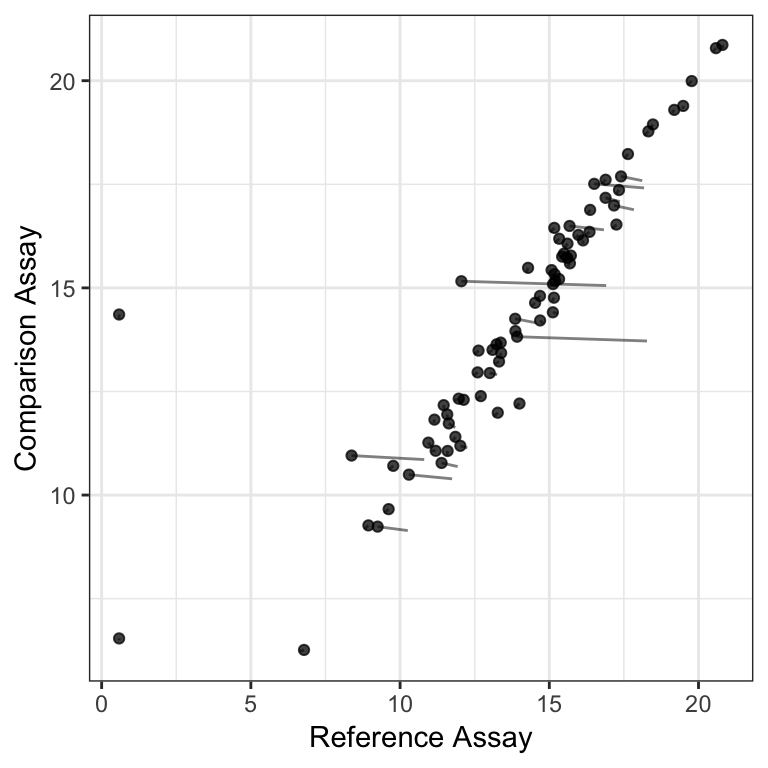
\includegraphics[width=\maxwidth]{figure/splitbyncells-1} \end{adjustwidth}
\end{knitrout}

The filtering function has several other options, including whether the filter shuld be applied (thus returning a new \sca object) or returned as a matrix of boolean values.

\begin{knitrout}
\definecolor{shadecolor}{rgb}{0.941, 0.941, 0.941}\color{fgcolor}\begin{kframe}
\begin{alltt}
\hlstd{vbeta.fa}
\end{alltt}
\begin{verbatim}
## class: FluidigmAssay 
## dim: 75 456 
## metadata(0):
## assays(1): Et
## rownames(75): B3GAT1 BAX ... TNFRSF9 TNFSF10
## rowData names(2): Gene primerid
## colnames(456): Sub01 1 A01 Sub01 1 A02 ... Sub02 3 H10 Sub02 3 H11
## colData names(9): Number.of.Cells Population ... Time wellKey
\end{verbatim}
\begin{alltt}
\hlcom{## Split by 'ncells', apply to each component, then recombine}
\hlstd{vbeta.filtered} \hlkwb{<-} \hlkwd{filter}\hlstd{(vbeta.fa,} \hlkwc{groups}\hlstd{=}\hlstr{'ncells'}\hlstd{)}
\hlcom{## Returned as boolean matrix}
\hlstd{was.filtered} \hlkwb{<-} \hlkwd{filter}\hlstd{(vbeta.fa,} \hlkwc{apply_filter}\hlstd{=}\hlnum{FALSE}\hlstd{)}
\hlcom{## Wells filtered for being discrete outliers}
\hlkwd{head}\hlstd{(}\hlkwd{subset}\hlstd{(was.filtered, pctout))}
\end{alltt}
\begin{verbatim}
##             intout null pctout
## Sub01 1 D05  FALSE TRUE   TRUE
## Sub01 1 D06  FALSE TRUE   TRUE
## Sub01 1 D07  FALSE TRUE   TRUE
## Sub01 1 D08  FALSE TRUE   TRUE
## Sub01 1 D10  FALSE TRUE   TRUE
## Sub01 1 D11  FALSE TRUE   TRUE
\end{verbatim}
\end{kframe}
\end{knitrout}

There's also some functionality for visualizing the filtering.

\begin{knitrout}
\definecolor{shadecolor}{rgb}{0.941, 0.941, 0.941}\color{fgcolor}\begin{kframe}
\begin{alltt}
\hlkwd{burdenOfFiltering}\hlstd{(vbeta.fa,} \hlstr{'ncells'}\hlstd{,} \hlkwc{byGroup}\hlstd{=}\hlnum{TRUE}\hlstd{)}
\end{alltt}
\end{kframe}\begin{adjustwidth}{\fltoffset}{0mm}
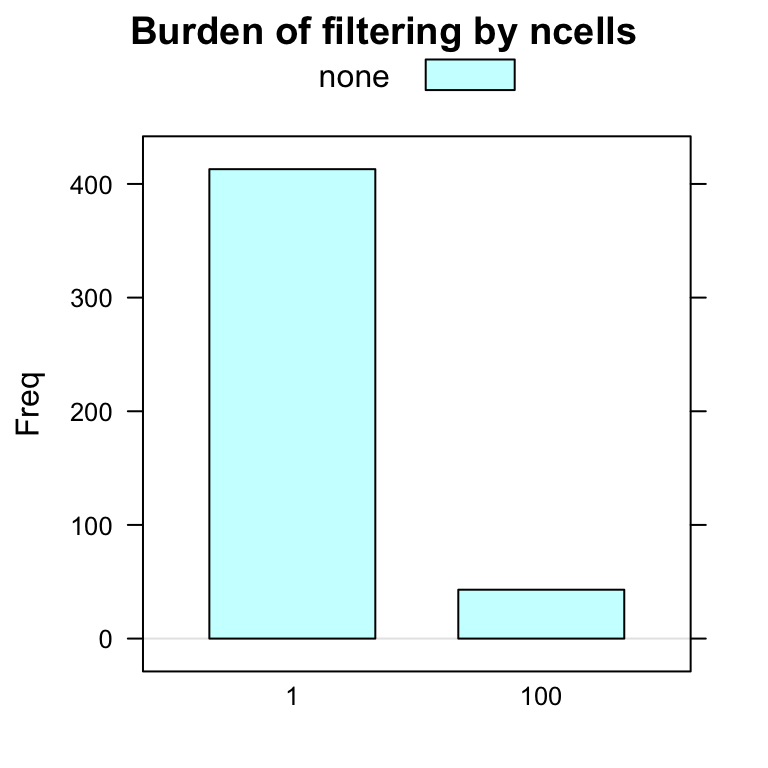
\includegraphics[width=\maxwidth]{figure/burdenOfFiltering-1} \end{adjustwidth}
\end{knitrout}


\section{Significance testing under the Hurdle model}
There are two frameworks available in the package.  The first framework \texttt{zlm} offers a full linear model to allow arbitrary comparisons and adjustment for covariates. The second framework \texttt{LRT} can be considered essentially performing t-tests (respecting the discrete/continuous nature of the data) between pairs of groups.  \texttt{LRT} is subsumed by the first framework, but might be simpler for some users, so has been kept in the package.

We'll describe \texttt{zlm}.  Models are specified in terms of the variable used as the measure and covariates present in the \texttt{cellData} using symbolic notation, just as the \texttt{lm} function in R.
\begin{knitrout}
\definecolor{shadecolor}{rgb}{0.941, 0.941, 0.941}\color{fgcolor}\begin{kframe}
\begin{alltt}
\hlstd{vbeta.1} \hlkwb{<-} \hlkwd{subset}\hlstd{(vbeta.fa, ncells}\hlopt{==}\hlnum{1}\hlstd{)}
\hlcom{## Consider the first 20 genes}
\hlstd{vbeta.1} \hlkwb{<-} \hlstd{vbeta.1[}\hlnum{1}\hlopt{:}\hlnum{20}\hlstd{,]}
\hlkwd{head}\hlstd{(}\hlkwd{colData}\hlstd{(vbeta.1))}
\end{alltt}
\begin{verbatim}
## DataFrame with 6 rows and 9 columns
##             Number.of.Cells            Population    ncells Subject.ID
##                   <integer>           <character> <integer>   <factor>
## Sub01 1 A01               1 CD154+VbetaResponsive         1      Sub01
## Sub01 1 A02               1 CD154+VbetaResponsive         1      Sub01
## Sub01 1 A03               1 CD154+VbetaResponsive         1      Sub01
## Sub01 1 A04               1 CD154+VbetaResponsive         1      Sub01
## Sub01 1 A05               1 CD154+VbetaResponsive         1      Sub01
## Sub01 1 A06               1 CD154+VbetaResponsive         1      Sub01
##             Chip.Number        Well Stim.Condition     Time     wellKey
##               <integer> <character>    <character> <factor> <character>
## Sub01 1 A01           1         A01      Stim(SEB)       12 Sub01 1 A01
## Sub01 1 A02           1         A02      Stim(SEB)       12 Sub01 1 A02
## Sub01 1 A03           1         A03      Stim(SEB)       12 Sub01 1 A03
## Sub01 1 A04           1         A04      Stim(SEB)       12 Sub01 1 A04
## Sub01 1 A05           1         A05      Stim(SEB)       12 Sub01 1 A05
## Sub01 1 A06           1         A06      Stim(SEB)       12 Sub01 1 A06
\end{verbatim}
\end{kframe}
\end{knitrout}
Now, for each gene, we can regress on \texttt{Et} the factors \texttt{Population} and \texttt{Subject.ID}.

In each gene, we'll fit a Hurdle model with a separate intercept for each population and subject.
A an S4 object of class ``ZlmFit'' is returned, containing slots with the genewise coefficients, variance-covariance matrices, etc.
\begin{knitrout}
\definecolor{shadecolor}{rgb}{0.941, 0.941, 0.941}\color{fgcolor}\begin{kframe}
\begin{alltt}
\hlkwd{library}\hlstd{(ggplot2)}
\hlstd{zlm.output} \hlkwb{<-} \hlkwd{zlm}\hlstd{(}\hlopt{~} \hlstd{Population} \hlopt{+} \hlstd{Subject.ID, vbeta.1,)}
\hlkwd{show}\hlstd{(zlm.output)}
\end{alltt}
\begin{verbatim}
## Fitted zlm on 20 genes and 413 cells.
##  Using BayesGLMlike ~ Population + Subject.ID
\end{verbatim}
\begin{alltt}
\hlcom{## returns a data.table with a summary of the fit}
\hlstd{coefAndCI} \hlkwb{<-} \hlkwd{summary}\hlstd{(zlm.output,} \hlkwc{logFC}\hlstd{=}\hlnum{FALSE}\hlstd{)}\hlopt{$}\hlstd{datatable}
\hlstd{coefAndCI} \hlkwb{<-} \hlstd{coefAndCI[contrast} \hlopt{!=} \hlstr{'(Intercept)'}\hlstd{,]}
\hlstd{coefAndCI[,contrast}\hlkwb{:=}\hlkwd{abbreviate}\hlstd{(contrast)]}
\hlkwd{ggplot}\hlstd{(coefAndCI,} \hlkwd{aes}\hlstd{(}\hlkwc{x}\hlstd{=contrast,} \hlkwc{y}\hlstd{=coef,} \hlkwc{ymin}\hlstd{=ci.lo,} \hlkwc{ymax}\hlstd{=ci.hi,} \hlkwc{col}\hlstd{=component))}\hlopt{+}
    \hlkwd{geom_pointrange}\hlstd{(}\hlkwc{position}\hlstd{=}\hlkwd{position_dodge}\hlstd{(}\hlkwc{width}\hlstd{=}\hlnum{.5}\hlstd{))} \hlopt{+}\hlkwd{facet_wrap}\hlstd{(}\hlopt{~}\hlstd{primerid)} \hlopt{+}
    \hlkwd{theme}\hlstd{(}\hlkwc{axis.text.x}\hlstd{=}\hlkwd{element_text}\hlstd{(}\hlkwc{angle}\hlstd{=}\hlnum{45}\hlstd{,} \hlkwc{hjust}\hlstd{=}\hlnum{1}\hlstd{))} \hlopt{+} \hlkwd{coord_cartesian}\hlstd{(}\hlkwc{ylim}\hlstd{=}\hlkwd{c}\hlstd{(}\hlopt{-}\hlnum{3}\hlstd{,} \hlnum{3}\hlstd{))}
\end{alltt}
\end{kframe}\begin{adjustwidth}{\fltoffset}{0mm}
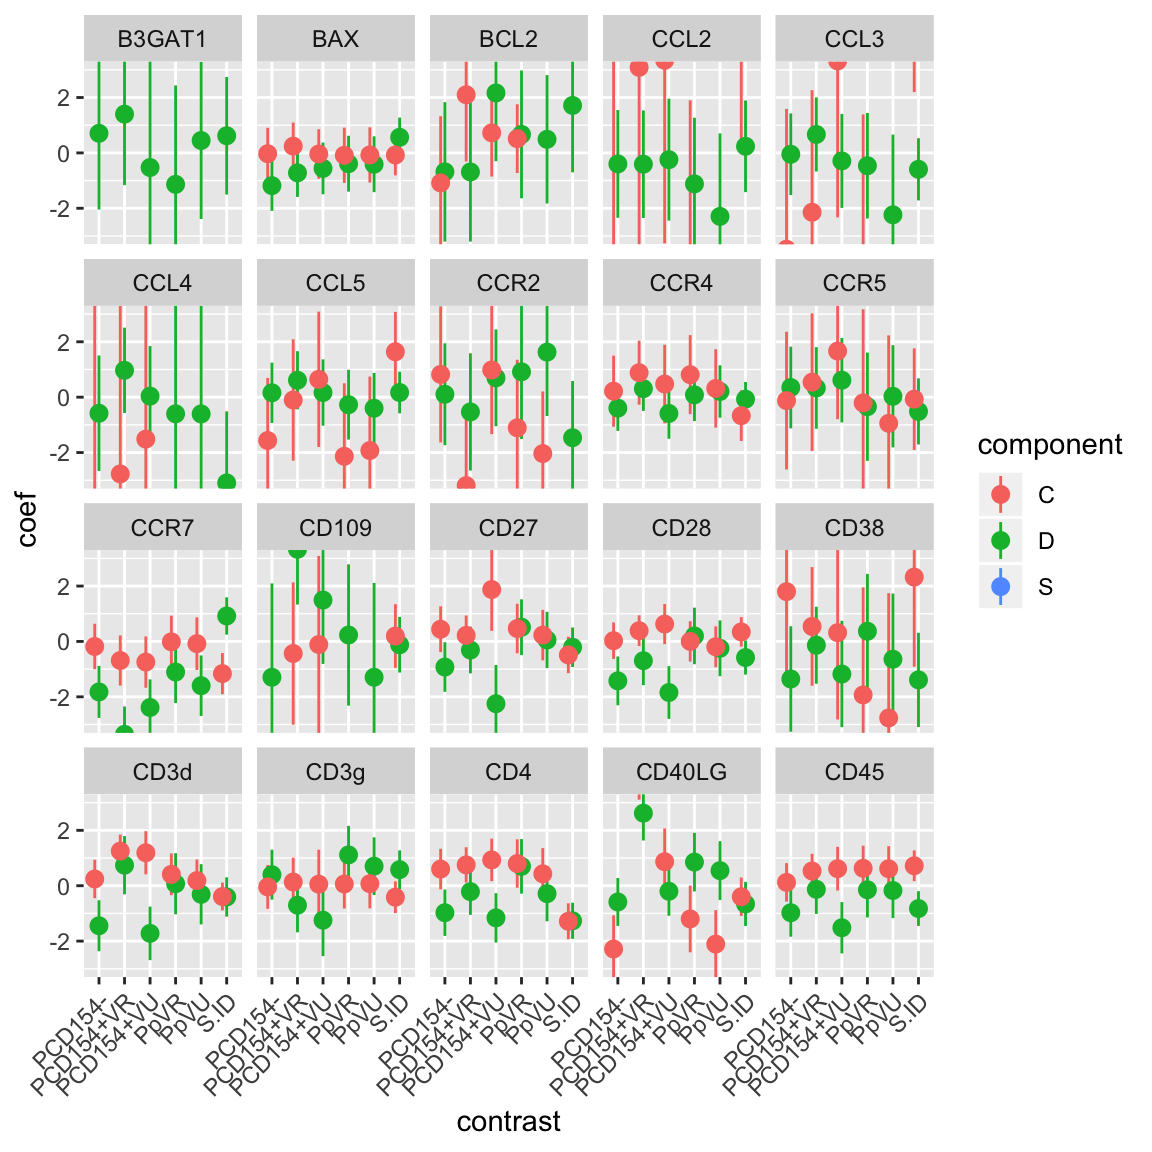
\includegraphics[width=\maxwidth]{figure/zlmExample-1} \end{adjustwidth}
\end{knitrout}
Try \verb|?ZlmFit-class| or \verb|showMethods(classes='ZlmFit')| to see a full list of methods. Multicore support is offered by setting \texttt{options(mc.cores=4)}, or however many cores your system has.

The combined test for differences in proportion expression/average expression is found by calling a likelihood ratio test on the fitted object.
An array of genes, metrics and test types is returned.
We'll plot the -log10 P values by gene and test type.
\begin{knitrout}
\definecolor{shadecolor}{rgb}{0.941, 0.941, 0.941}\color{fgcolor}\begin{kframe}
\begin{alltt}
\hlstd{zlm.lr} \hlkwb{<-} \hlkwd{lrTest}\hlstd{(zlm.output,} \hlstr{'Population'}\hlstd{)}
\end{alltt}


{\ttfamily\noindent\itshape\color{messagecolor}{\#\# Refitting on reduced model...}}

{\ttfamily\noindent\itshape\color{messagecolor}{\#\# .\\\#\# Done!}}\begin{alltt}
\hlkwd{dimnames}\hlstd{(zlm.lr)}
\end{alltt}
\begin{verbatim}
## $primerid
##  [1] "B3GAT1" "BAX"    "BCL2"   "CCL2"   "CCL3"   "CCL4"   "CCL5"   "CCR2"  
##  [9] "CCR4"   "CCR5"   "CCR7"   "CD109"  "CD27"   "CD28"   "CD38"   "CD3d"  
## [17] "CD3g"   "CD4"    "CD40LG" "CD45"  
## 
## $test.type
## [1] "cont"   "disc"   "hurdle"
## 
## $metric
## [1] "lambda"     "df"         "Pr(>Chisq)"
\end{verbatim}
\begin{alltt}
\hlstd{pvalue} \hlkwb{<-} \hlkwd{ggplot}\hlstd{(}\hlkwd{melt}\hlstd{(zlm.lr[,,}\hlstr{'Pr(>Chisq)'}\hlstd{]),} \hlkwd{aes}\hlstd{(}\hlkwc{x}\hlstd{=primerid,} \hlkwc{y}\hlstd{=}\hlopt{-}\hlkwd{log10}\hlstd{(value)))}\hlopt{+}
    \hlkwd{geom_bar}\hlstd{(}\hlkwc{stat}\hlstd{=}\hlstr{'identity'}\hlstd{)}\hlopt{+}\hlkwd{facet_wrap}\hlstd{(}\hlopt{~}\hlstd{test.type)} \hlopt{+} \hlkwd{coord_flip}\hlstd{()}
\hlkwd{print}\hlstd{(pvalue)}
\end{alltt}
\end{kframe}\begin{adjustwidth}{\fltoffset}{0mm}
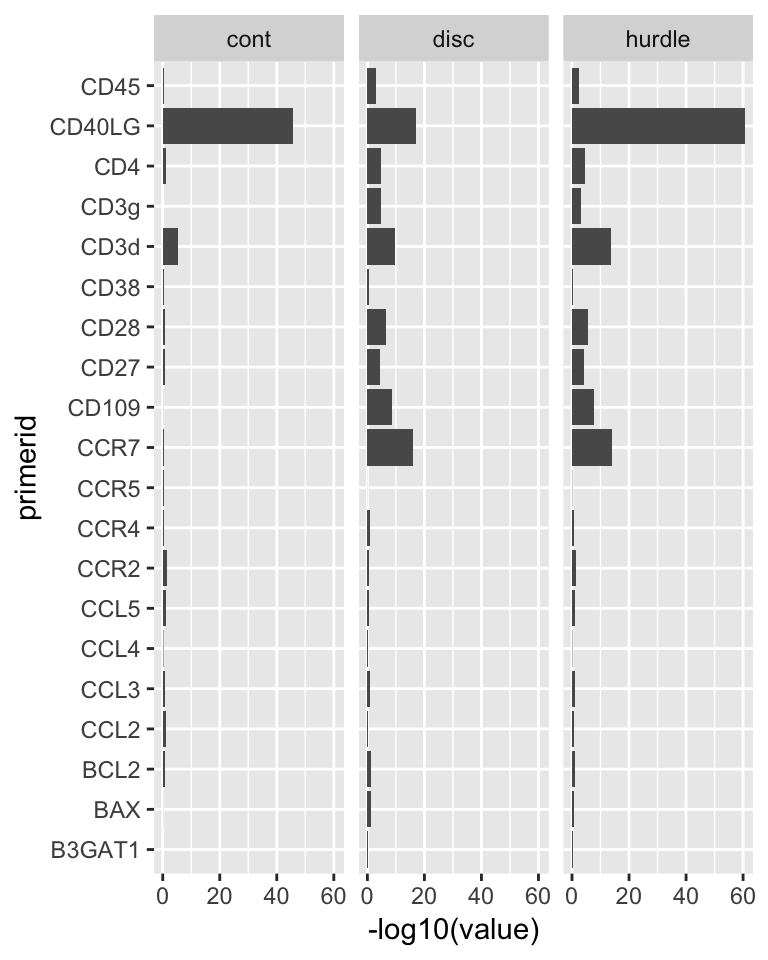
\includegraphics[width=\maxwidth]{figure/tests-1} \end{adjustwidth}
\end{knitrout}

In fact, the \texttt{zlm} framework is quite general, and has wrappers for a variety of  modeling functions that accept \texttt{glm}-like arguments to be used, such as mixed models (using \texttt{lme4}).
%This is not eval'd because of mysterious errors emanating from lme4 on the bioconductor machines that I am unable to reproduce.
% Warning: failed to assign RegisteredNativeSymbol for deepcopy to deepcopy since deepcopy is already defined in the 'lme4' namespace
% Quitting from lines 230-232 (MAST-intro.Rnw) 
% Error: processing vignette 'MAST-intro.Rnw' failed with diagnostics:
% first argument must be a string (of length 1) or native symbol reference
% Execution halted
\begin{knitrout}
\definecolor{shadecolor}{rgb}{0.941, 0.941, 0.941}\color{fgcolor}\begin{kframe}
\begin{alltt}
\hlkwd{library}\hlstd{(lme4)}
\hlstd{lmer.output} \hlkwb{<-} \hlkwd{zlm}\hlstd{(}\hlopt{~} \hlstd{Stim.Condition} \hlopt{+}\hlstd{(}\hlnum{1}\hlopt{|}\hlstd{Subject.ID), vbeta.1,} \hlkwc{method}\hlstd{=}\hlstr{'glmer'}\hlstd{,} \hlkwc{ebayes}\hlstd{=}\hlnum{FALSE}\hlstd{)}
\end{alltt}
\end{kframe}
\end{knitrout}

By default, we employ Bayesian logistic regression, which imposes a Cauchy prior of the regression coefficients, for the discrete component.  This provides reasonable inference under linear separation.
We default to regular least squares for the continuous component with an empirical Bayes' adjustment for the dispersion (variance) estimate.
However, the prior can be adjusted (see \texttt{defaultPrior}) or eliminated entirely by setting \texttt{method='glm'} in \texttt{zlm}.
It is also possible to use Bayesian linear regression for the continuous component by setting \texttt{useContinuousBayes=TRUE} in \texttt{zlm}.
For example:
\begin{knitrout}
\definecolor{shadecolor}{rgb}{0.941, 0.941, 0.941}\color{fgcolor}\begin{kframe}
\begin{alltt}
 \hlstd{orig_results} \hlkwb{<-} \hlkwd{zlm}\hlstd{(}\hlopt{~}\hlstd{Stim.Condition, vbeta.1)}
 \hlstd{dp} \hlkwb{<-} \hlkwd{defaultPrior}\hlstd{(}\hlstr{'Stim.ConditionUnstim'}\hlstd{)}
 \hlstd{new_results} \hlkwb{<-}  \hlkwd{zlm}\hlstd{(}\hlopt{~}\hlstd{Stim.Condition, vbeta.1,} \hlkwc{useContinuousBayes}\hlstd{=}\hlnum{TRUE}\hlstd{,}\hlkwc{coefPrior}\hlstd{=dp)}
 \hlkwd{qplot}\hlstd{(}\hlkwc{x}\hlstd{=}\hlkwd{coef}\hlstd{(orig_results,} \hlstr{'C'}\hlstd{)[,} \hlstr{'Stim.ConditionUnstim'}\hlstd{],}
       \hlkwc{y}\hlstd{=}\hlkwd{coef}\hlstd{(new_results,} \hlstr{'C'}\hlstd{)[,} \hlstr{'Stim.ConditionUnstim'}\hlstd{],}
       \hlkwc{color}\hlstd{=}\hlkwd{coef}\hlstd{(new_results,} \hlstr{'D'}\hlstd{)[,}\hlstr{'(Intercept)'}\hlstd{])} \hlopt{+}
     \hlkwd{xlab}\hlstd{(}\hlstr{'Default prior'}\hlstd{)} \hlopt{+} \hlkwd{ylab}\hlstd{(}\hlstr{'Informative Prior'}\hlstd{)} \hlopt{+}
     \hlkwd{geom_abline}\hlstd{(}\hlkwc{slope}\hlstd{=}\hlnum{1}\hlstd{,} \hlkwc{lty}\hlstd{=}\hlnum{2}\hlstd{)} \hlopt{+} \hlkwd{scale_color_continuous}\hlstd{(}\hlstr{'Baseline\textbackslash{}nlog odds\textbackslash{}nof expression'}\hlstd{)}
\end{alltt}
\end{kframe}\begin{adjustwidth}{\fltoffset}{0mm}
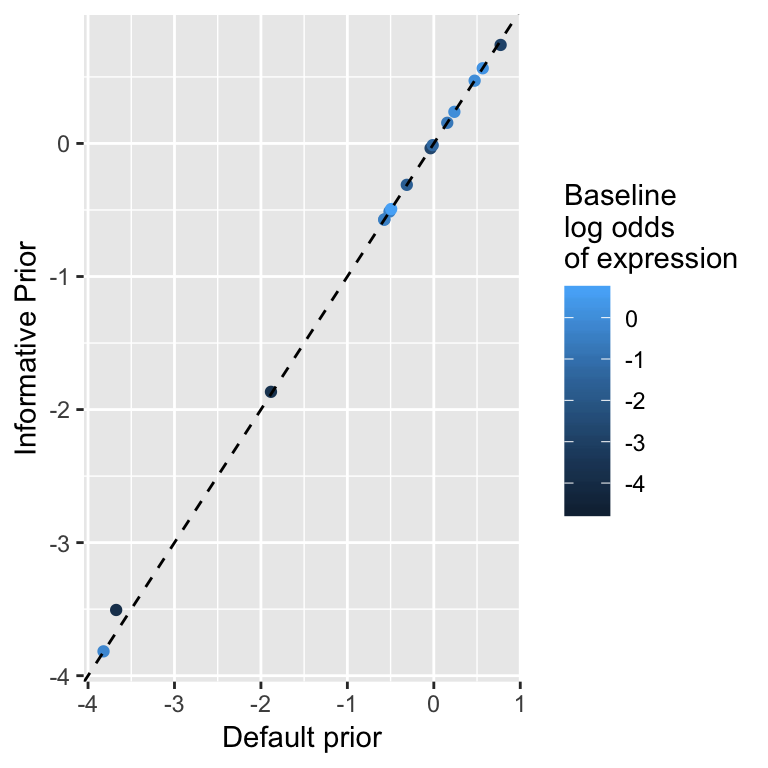
\includegraphics[width=\maxwidth]{figure/advancedArmExample-1} \end{adjustwidth}
\end{knitrout}
After applying a prior to the continuous component, its estimates are shrunken towards zero, with the amount of shrinkage inversely depending on the number of expressing cells in the gene.



\subsection{Two-sample Likelihood Ratio Test}
  Another way to test for differential expression is available through
  the \texttt{LRT} function, which is analogous to two-sample T tests.
\begin{knitrout}
\definecolor{shadecolor}{rgb}{0.941, 0.941, 0.941}\color{fgcolor}\begin{kframe}
\begin{alltt}
\hlstd{two.sample} \hlkwb{<-} \hlkwd{LRT}\hlstd{(vbeta.1,} \hlstr{'Population'}\hlstd{,} \hlkwc{referent}\hlstd{=}\hlstr{'CD154+VbetaResponsive'}\hlstd{)}
\hlkwd{head}\hlstd{(two.sample)}
\end{alltt}
\begin{verbatim}
##              Population test.type primerid    lrstat direction   p.value
## 1 CD154-VbetaResponsive      comb   B3GAT1 1.5722257        -1 0.4556124
## 2 CD154-VbetaResponsive      comb      BAX 1.5847859         1 0.4527601
## 3 CD154-VbetaResponsive      comb     BCL2 0.7821003        -1 0.6763462
## 4 CD154-VbetaResponsive      comb     CCL2 3.3431031        -1 0.1879552
## 5 CD154-VbetaResponsive      comb     CCL3 0.1401862        -1 0.9323070
## 6 CD154-VbetaResponsive      comb     CCL4 0.6305951         1 0.7295718
\end{verbatim}
\end{kframe}
\end{knitrout}

Here we compare each population (\texttt{CD154-VbetaResponsive, CD154-VbetaUnresponsive CD154+VbetaUnresponsive, VbetaResponsive, VbetaUnresponsive}) to the \texttt{CD154+VbetaResponsive} population.
  The \texttt{Population} column shows which population is being
  compared, while \texttt{test.type} is \texttt{comb} for the combined
  normal theory/binomial test.  Column \texttt{primerid} gives the
  gene being tested, \texttt{direction} shows if the comparison group
  mean is greater (1) or less (-1) than the referent group, and
  \texttt{lrtstat} and \texttt{p.value} give the test statistic and
  $\chi^2$ p-value (two degrees of freedom).
Other options are whether additional information about the tests are
returned (\texttt{returnall=TRUE}) and if the testing should be
stratified by a character vector naming columns in \texttt{colData} 
containing grouping variables (\texttt{groups}).

These tests have been subsumed by \texttt{zlm} but
remain in the package for user convenience.

\section{Use with single cell RNA-sequencing data}
In RNA-sequencing data is essentially no different than qPCR-based single cell gene expression, once it has been aligned and mapped, if one is willing to reduce the experiment to counts or count-like data for a fixed set of genes/features.  
We assume that suitable tools (eg, RSEM, Kallisto or TopHat) have been applied to do this.

An example of this use is provided in a vignette.  Type \texttt{vignette('MAITAnalysis')} to view.
\begin{comment}
  \section{Implementation Details}
  Here we provide some background on the implementation of the
  package.

  There are several fundamental new object types provided by the
  package.  \texttt{SummarizedExperiment} is the base class, which is
  provides an array-like object to store tabular data that might have
  multiple derived representations. 
  On construction of a \texttt{SingleCellAssay} object, the package
  tests for completeness, and will fill in the missing data (with NA)
  if it is not, so assays with lots of missing data can make reading
  marginally slower.
\end{comment}
\end{document}
